% Provenance (never printed): old terminale S material on past climates (ice cores,
% pollen, ocean sediments and oxygen isotopes, glacial-interglacial cycles, the
% astronomical rhythm told, climates of deep time), read from data. Owner (Sync 0/1):
% climate archive and proxy, ice core, glacial period, interglacial and glacial cycle,
% pollen analysis, Last Glacial Maximum. Recalled: glacier, ice sheet, ice age (Book 1,
% grade 8); the first look at the ice-core records (Book 1, grade 9); isotopes
% (physics); greenhouse gases (chemistry); the time scale (Book 1, grade 7). The
% delta notation of isotopes is Book 3's: isotope curves are read here as told,
% without a definition. The orbital theory of climate belongs to a university book:
% told here only. Physical science only, in the IPCC's calibrated words.
% Figures: figdata/grade-12/ice_age_records.py (tests/grade-12/test_ice_age_records.py).
\chapter{قراءة المناخات الماضية}\label{ch:g12:past-climates}

في دوم~C، على ارتفاع \qty{3233}{m} فوق الغطاء الجليدي لشرق القارة القطبية الجنوبية، يبلغ
متوسط درجة حرارة الهواء نحو \qty{-55}{\degreeCelsius} على مدار السنة. وقد توقف حفّار يعمل هناك
عند عمق \qty{3260}{m}، على بعد نحو \qty{15}{m} فوق الصخر الذي تحت
الجليد. ويحوي أعمق جليد استخرجه فقاعات صغيرة من هواء يبلغ عمره نحو
\num{800000} سنة: عينة من الغلاف الجوي من زمن يسبق كثيرًا
المزارعين الأوائل. يقرأ هذا الفصل
مناخ الماضي في الجليد، وفي وحل البحيرات وقاع
المحيط، وفي الصخور، ويسأل عما يقوله عن حاضرنا.
% ledger: ipev:concordia, edc3:drilling, jouzel07:edc

\begin{omfigure}
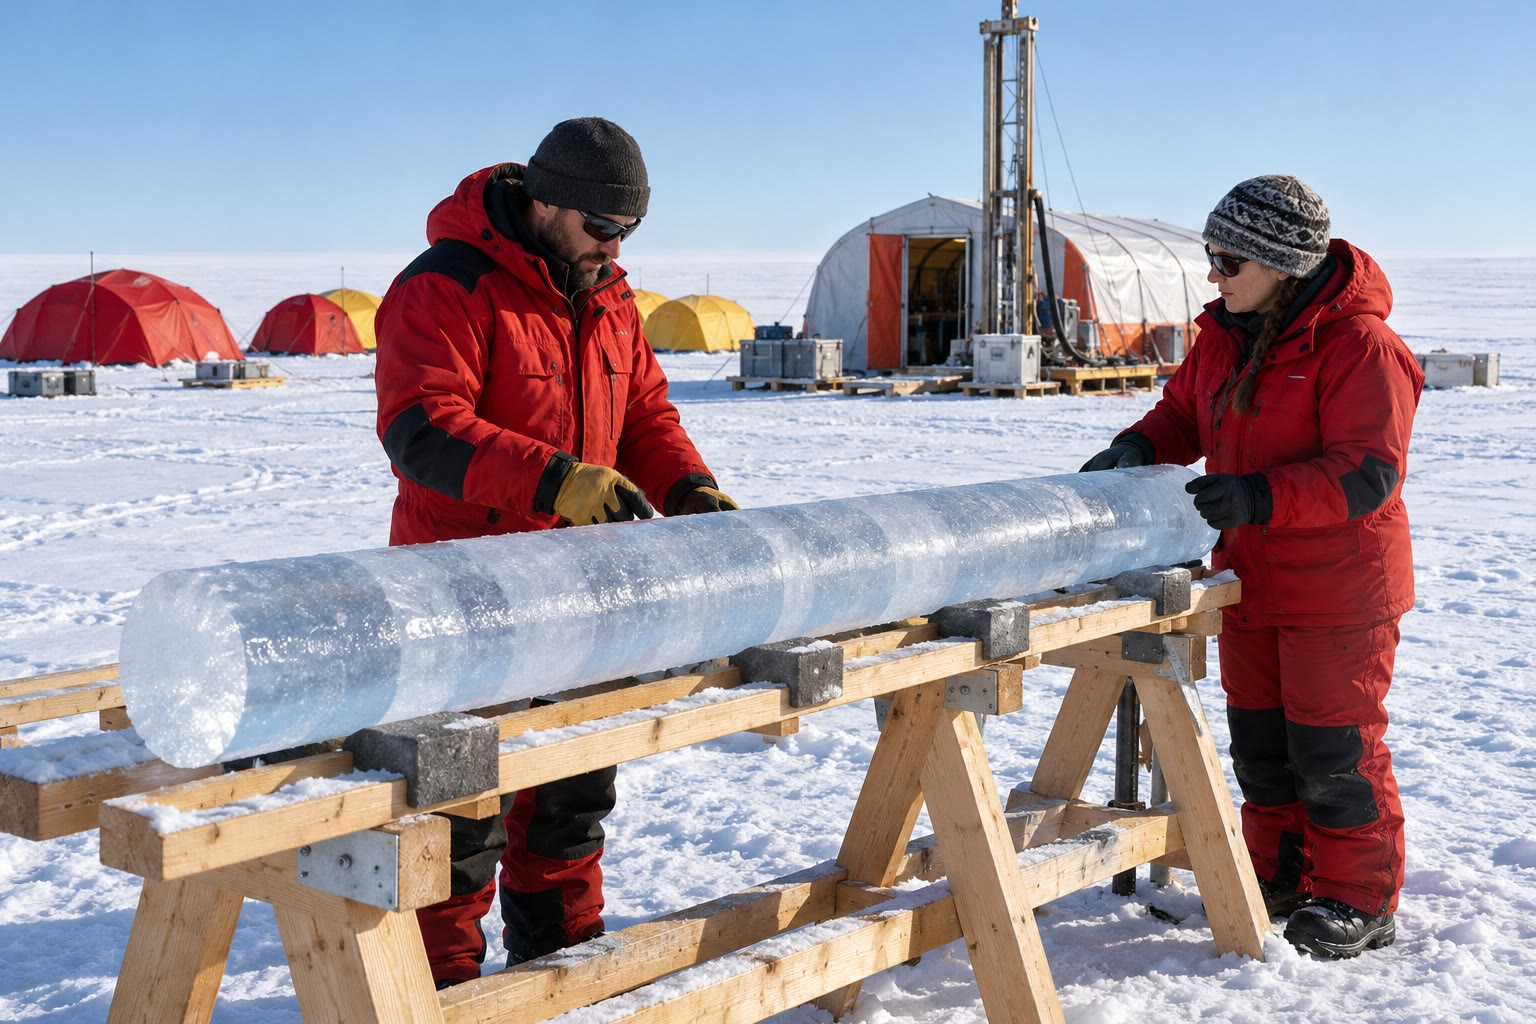
\includegraphics[width=0.56\linewidth]{images/book2/ai/g12-ice-coring-camp.jpg}

{\small مخيم لحفر \omterm{def:g12:past-climates:ice-core}{العينات الجليدية} على غطاء جليدي قطبي: يعمل الحفّار تحت
البرج والمأوى، ويُمدَّد كل جزء من العينة ويُسجَّل ويُعبَّأ
قبل أن يُنقل إلى المختبر. رسم توضيحي مولَّد بالذكاء الاصطناعي.}
\end{omfigure}

\begin{recall}
النهر الجليدي كتلة من الجليد تبقى من سنة إلى سنة وتنساب تحت
ثقلها؛ والغطاء الجليدي يغطي جزءًا كبيرًا من قارة؛ والعصر الجليدي
زمن بارد طويل تمتد فيه الأغطية الجليدية بعيدًا وراء القطبين (الكتاب 1، الصف 8).
وفي \omterm{def:g12:past-climates:ice-core}{العينات الجليدية} من القارة القطبية الجنوبية، يسجل الثلج درجة حرارة الهواء وتحفظ
الفقاعات الهواء نفسه، ويرتفع السجلان وينخفضان معًا
(الكتاب 1، الصف 9). وقد تختلف ذرات العنصر الواحد في عدد
نيوتروناتها: فهذه النظائر تتصرف تصرفًا متشابهًا في الكيمياء لكنها تختلف في الكتلة (كتب
الفيزياء). وثاني أكسيد الكربون غاز دفيئة (كتب الكيمياء).
وقد بدأ العصر الرابعي قبل 2.58 مليون سنة
(الكتاب 1، الصف 7).
\end{recall}
% ledger: ics:base.Quaternary (shared), nasaeo:o18 (snow poor in heavy isotopes)

\section{الأرشيفات والمؤشرات البديلة}

لم يقس أحد درجة حرارة الهواء قبل \num{20000} سنة. لكن
الأرض احتفظت بسجلات دون قصد: طبقات من الجليد والوحل، وأصداف وجذوع
أشجار، تغيّر كل منها مع المناخ الذي تكوّن فيه.

\begin{definition}[الأرشيف المناخي؛ المؤشر البديل]\label{def:g12:past-climates:proxy}
\emph{الأرشيف المناخي}\index{أرشيف مناخي} مادة طبيعية تترسب
في طبقات، واحدة تلو الأخرى، فتحتفظ بأثر من مناخ
الزمن الذي تكوّنت فيه: الجليد القطبي، ورسوبيات البحيرات وقاع المحيط،
وحلقات الأشجار، والمرجان، ورواسب الكهوف. و\emph{المؤشر البديل}\index{مؤشر بديل}
كمية تُقاس في أرشيف وتقوم مقام متغير مناخي لم
يُقس: حصة النظائر الثقيلة في الثلج القديم بدلًا من درجة حرارة
الهواء، وحصة كل نوع من حبوب اللقاح في وحل البحيرات بدلًا من الغطاء النباتي
ومن ثم المناخ.
\end{definition}
% ledger: ncei:proxy, ncei:pollen, nasaeo:o18

\begin{center}
\small
\begin{tabular}{|l|l|l|}
\hline
\textbf{الأرشيف} & \textbf{\omterm{def:g12:past-climates:proxy}{المؤشر البديل}} & \textbf{ما يخبر عنه} \\
\hline
الجليد القطبي & النظائر الثقيلة في الجليد & درجة حرارة الهواء فوق الجليد \\
 & الهواء في الفقاعات & ثاني أكسيد الكربون، والميثان \\
رسوبيات البحيرات، والخث & حبوب اللقاح & الغطاء النباتي، ثم المناخ \\
رسوبيات المحيطات & نظائر الأكسجين في الأصداف & حجم الجليد، ودرجة حرارة المياه العميقة \\
حلقات الأشجار & عرض الحلقة & ظروف النمو، سنة بسنة \\
المرجان، ورواسب الكهوف & النظائر، وأشرطة النمو & درجة حرارة البحر أو الهواء، والمطر \\
\hline
\end{tabular}

\medskip
{\small أهم الأرشيفات المناخية وبعض مؤشراتها البديلة.}
\end{center}
% ledger: ncei:proxy, nasaeo:o18

كل \omterm{def:g12:past-climates:proxy}{مؤشر بديل} يحتاج إلى أمرين قبل أن يمكن قراءته. فهو يحتاج إلى \emph{ساعة}:
عمر كل طبقة، بعدّ الطبقات السنوية حيث يمكن رؤيتها،
أو بالتأريخ الإشعاعي (\cref{ch:g12:age-of-the-earth})، أو بمطابقة
السجل مع سجل آخر مؤرَّخ من قبل. ويحتاج إلى \emph{معايرة}: أي
الصلة بين ما يُقاس والمتغير المناخي، تُستخرج اليوم، حيث
يمكن قياس الاثنين معًا.

\begin{method}[قراءة سجل مؤشر بديل]
\begin{enumerate}
  \item جد الأرشيف \omterm{def:g12:past-climates:proxy}{والمؤشر البديل}: ماذا قيس، وفي أي مادة؟
  \item جد الاتجاه الذي يجري فيه الزمن على المحور، وبأي وحدة؛ وتحقق
        مما إذا كان محور \omterm{def:g12:past-climates:proxy}{المؤشر البديل} معكوسًا.
  \item ترجم \omterm{def:g12:past-climates:proxy}{المؤشر البديل}: هل القيمة الأعلى تعني أدفأ أم أبرد،
        وجليدًا أكثر أم أقل؟
  \item لاحظ تباعد العينات: فالسجل الذي تتباعد نقاطه
        \num{2000} سنة لا يستطيع أن يُظهر تغيرًا دام قرنًا.
  \item اقرأ القيم عند التواريخ المطلوبة، أو المتوسطات على فترة،
        واحسب التغيرات والمعدلات.
  \item قل ما يُظهره السجل في موقعه، ثم بعد ذلك فقط هل
        يمثل الأرض كلها.
\end{enumerate}
\end{method}

\section{العينات الجليدية}

\begin{definition}[العينة الجليدية]\label{def:g12:past-climates:ice-core}
\emph{العينة الجليدية}\index{عينة جليدية} أسطوانة من الجليد تُستخرج بالحفر من غطاء
جليدي أو نهر جليدي. يعطي عمقها عمر الجليد، فكلما كان أعمق كان أقدم؛
ويسجل الجليد درجة حرارة الهواء الذي سقط فيه ثلجه، وتحفظ
فقاعاته عينات من هواء ذلك الزمن.
\end{definition}
% ledger: ncei:proxy, jouzel07:edc

الثلج الطازج في معظمه هواء. وحين يُدفن تحت ثلج السنوات التالية،
يُضغط فيصير \emph{فِرنًا}، وهو ثلج متراص لا تزال مسامه تمرر الهواء.
وعند كثافة تبلغ نحو 820 إلى \qty{830}{kg/m^3}، تُبلغ على عمق 50 إلى \qty{120}{m}،
تنغلق المسام ويُحبس الهواء في فقاعات. وهكذا يحفظ الجليد سجلين
مختلفين. فالهواء في الفقاعات عينة من الغلاف الجوي، يُقاس ما فيها من ثاني أكسيد
الكربون والميثان في المختبر. أما الجليد نفسه فيحفظ
درجة الحرارة: فجزيئات الماء التي تحوي نظيرًا ثقيلًا (الديوتيريوم أو
الأكسجين-18) تتكاثف أسهل من الخفيفة، فكلما برد الهواء
في طريقه إلى القطب، فقُر الثلج بالنظائر الثقيلة.
% ledger: firn:close-off, nasaeo:o18

\begin{omfigure}
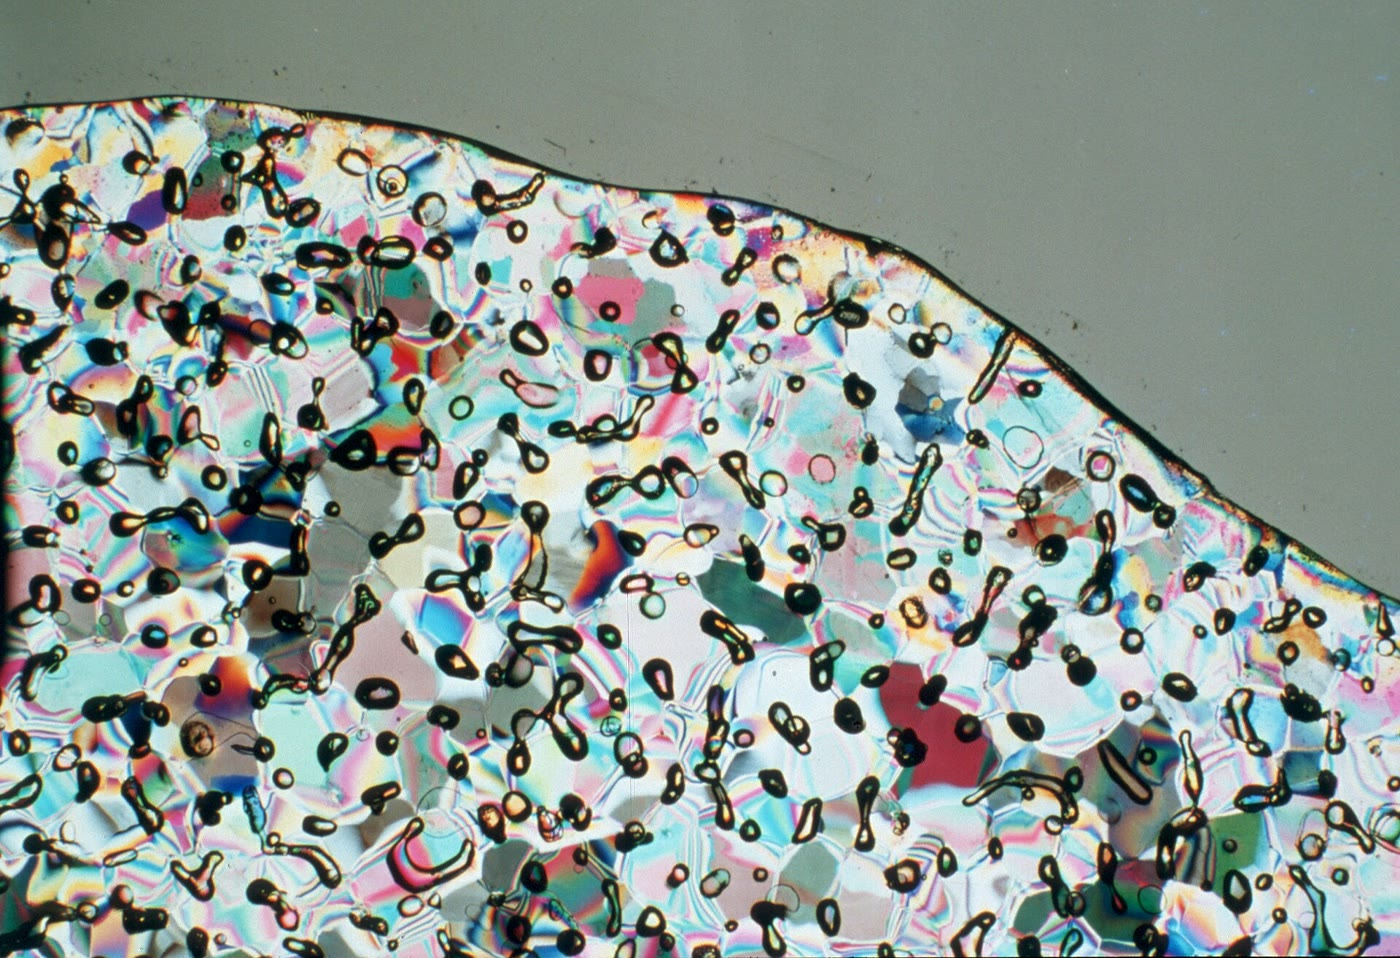
\includegraphics[width=0.50\linewidth]{images/book2/g12-ice-bubbles.jpg}

{\small شريحة من جليد القارة القطبية الجنوبية تحت ضوء مستقطب، يلوّن
بلورات الجليد: والنقاط الداكنة فقاعات من الهواء المحبوس. الصورة: منظمة الكومنولث
للبحث العلمي والصناعي، قسم أبحاث الغلاف الجوي، CC~BY~3.0 (ويكيميديا كومنز).}
\end{omfigure}
% ledger: photo:g12-ice-bubbles

حُوّل ديوتيريوم عينة دوم~C إلى درجة حرارة فوق
الجليد، تُعطى تغيرًا مقارنةً بمتوسط الألف سنة الأخيرة. أما
ثاني أكسيد الكربون فمأخوذ من فقاعات عدة \omterm{def:g12:past-climates:ice-core}{عينات جليدية} من القارة القطبية الجنوبية، جُمعت
في سجل واحد. وكلاهما مرسوم أدناه على محور زمني واحد.

\begin{omfigure}
\begin{tikzpicture}
\begin{axis}[omrecord, scale only axis, width=0.74\linewidth, height=4.8cm,
  xmin=0, xmax=800, x dir=reverse, ymin=-12, ymax=8, axis y line*=left,
  xtick={0,100,...,800}, ytick={-10,-5,0,5},
  xlabel={\foreignlanguage{arabic}{آلاف السنين قبل عام 1950}},
  ylabel={\foreignlanguage{arabic}{تغير درجة الحرارة \babelsublr{(\unit{\degreeCelsius})}}}]
% data:edc-jouzel, 2-kyr means (figdata/grade-12/ice_age_records.py)
\addplot[omWarm, line width=0.7pt] table[x=age_kyr, y=temp_C] {figdata/out/grade-12-ice_age_records-edc.dat};
\end{axis}
\begin{axis}[scale only axis, width=0.74\linewidth, height=4.8cm,
  xmin=0, xmax=800, x dir=reverse, ymin=60, ymax=320, axis y line*=right,
  axis x line=none, ytick={180,220,260,300}, ylabel={\foreignlanguage{arabic}{ثاني أكسيد الكربون \babelsublr{(ppm)}}},
  every axis label/.append style={font=\small}, tick label style={font=\small}]
% data:co2-bereiter, 2-kyr means
\addplot[black, line width=0.7pt] table[x=age_kyr, y=co2_ppm] {figdata/out/grade-12-ice_age_records-co2.dat};
\coordinate (lt) at (axis cs:560,70);
\coordinate (lc) at (axis cs:560,312);
\end{axis}
\node[font=\scriptsize, text=omWarm, anchor=south] at (lt) {\foreignlanguage{arabic}{درجة الحرارة في دوم~C، المقياس الأيسر}};
\node[font=\scriptsize, anchor=north] at (lc) {\foreignlanguage{arabic}{ثاني أكسيد الكربون، المقياس الأيمن}};
\end{tikzpicture}

{\small ثمانمئة ألف سنة من جليد القارة القطبية الجنوبية، بمتوسطات على خطوات من
\num{2000} سنة. بالأحمر: درجة الحرارة في دوم~C مقارنةً بالألف سنة
الأخيرة (جوزيل وآخرون، 2007)؛ وبالأسود: ثاني أكسيد الكربون في
الفقاعات (بيرايتر وآخرون، 2015). والحاضر في اليمين.}
\end{omfigure}
% ledger: data:edc-jouzel, data:co2-bereiter

يشترك المنحنيان في نمط واحد: انزلاق بطيء متعرج نحو البرد على مدى
عشرات آلاف السنين، ثم صعود سريع إلى الدفء، ثم
الانزلاق من جديد.

\begin{definition}[الفترة الجليدية؛ الفترة بين الجليدية؛ الدورة الجليدية]\label{def:g12:past-climates:glacial-cycle}
\emph{الفترة الجليدية}\index{فترة جليدية} فترة باردة داخل
عصر جليدي، تنمو فيها الأغطية الجليدية إلى ما يتجاوز حجمها الحالي بكثير.
و\emph{الفترة بين الجليدية}\index{فترة بين جليدية} فترة دافئة بين فترتين
جليديتين، تكون فيها الأغطية الجليدية قريبة من حجمها اليوم أو أصغر؛ ونحن نعيش في إحداها،
وقد بدأت قبل نحو \num{11000} سنة. و\emph{الدورة
الجليدية}\index{دورة جليدية} فترة جليدية واحدة مع الفترة بين الجليدية التي
تنهيها.
\end{definition}
% ledger: ipcc:ref-periods (LDT ends 11 ka); the count of cycles is read from the figure (data:edc-jouzel)

على امتداد السجل كله، تتراوح درجة الحرارة في دوم~C بين
\qty{-10.6}{\degreeCelsius}، قبل نحو \num{24000} سنة،
و\qty{+5.5}{\degreeCelsius}، قبل نحو \num{129000} سنة؛ ويتراوح ثاني أكسيد الكربون
بين \qty{174}{ppm} و\qty{299}{ppm}. والشكل، الذي تُحسب متوسطاته على \num{2000}
سنة، يُنعّم هذه القيم القصوى قليلًا. وعدّ قمم الدفء يعطي ثماني
أو تسع \omterm{def:g12:past-climates:glacial-cycle}{دورات جليدية}، وأقوى إيقاع في سجل درجة الحرارة،
محسوبًا من بياناته، دورته نحو \num{98000} سنة.
% ledger: data:edc-jouzel, data:co2-bereiter (ice_age_records.py: edc_min_C -10.58 at 24.0 kyr, edc_max_C 5.46 at 128.7 kyr, co2 173.71 and 298.6, edc_period_kyr 97.5)

\begin{proposition}[درجة الحرارة وثاني أكسيد الكربون يتغيران معًا]\label{prop:g12:past-climates:correlation}
% ledger: data:edc-jouzel, data:co2-bereiter (ice_age_records.py: r_temp_co2 0.9165, fit 266.57 + 7.827 T, 1639 pairs)
على مدى \num{800000} السنة الأخيرة، تغيرت درجة حرارة القارة القطبية الجنوبية وثاني أكسيد
الكربون في الهواء معًا. ومزاوجة كل قياس من قياسات ثاني أكسيد الكربون البالغة 1639
والأقدم من \num{2000} سنة مع درجة حرارة دوم~C عند
العمر نفسه تعطي معامل ارتباط $r = 0.92$،
وخط المربعات الصغرى
\[
  \mathrm{CO_2} \approx \qty{267}{ppm} + \qty{7.8}{ppm/\degreeCelsius} \times \Delta T ,
\]
حيث $\Delta T$ تغير درجة الحرارة في دوم~C.
\end{proposition}

\begin{proof}[كيف يُحسب]
لكل عينة من ثاني أكسيد الكربون، تُقرأ درجة الحرارة عند عمرها في
سجل دوم~C بالاستيفاء بين أقرب نقطتين من نقاط درجة الحرارة.
ويُحسب معامل الارتباط للأزواج البالغة 1639، وهو عدد بين $-1$ و$1$
يقيس مدى قرب النقاط من خط مستقيم (كتب
الرياضيات)، مع خط المربعات الصغرى؛ وكلاهما يُحسب في
برنامج الشكل ويتحقق منه اختباره.
\end{proof}

\begin{omfigure}
\begin{tikzpicture}
\begin{axis}[omrecord, width=0.70\linewidth, height=5.2cm, xmin=-12, xmax=6,
  ymin=160, ymax=310, xlabel={\foreignlanguage{arabic}{تغير درجة الحرارة في دوم~C \babelsublr{(\unit{\degreeCelsius})}}},
  ylabel={\foreignlanguage{arabic}{ثاني أكسيد الكربون \babelsublr{(ppm)}}}]
% data:edc-jouzel, data:co2-bereiter (pairs and fit in ice_age_records.py)
\addplot[only marks, mark=*, mark size=0.6pt, omDef, opacity=0.45] table[x=temp_C, y=co2_ppm] {figdata/out/grade-12-ice_age_records-pairs.dat};
\addplot[omThm, line width=1pt] table[x=temp_C, y=co2_ppm] {figdata/out/grade-12-ice_age_records-fit.dat};
\node[font=\scriptsize, text=omThm, anchor=south east, fill=white, inner sep=1pt] at (axis cs:-1.5,295) {\foreignlanguage{arabic}{خط المربعات الصغرى، $r = 0.92$}};
\end{axis}
\end{tikzpicture}

{\small كل نقطة قياس واحد لثاني أكسيد الكربون في جليد القارة القطبية الجنوبية،
موضوع عند درجة حرارة دوم~C للعمر نفسه: فالأزمنة الباردة كان فيها قليل من ثاني أكسيد
الكربون، والأزمنة الدافئة أكثر بكثير. حُسب من جوزيل وآخرين (2007)
وبيرايتر وآخرين (2015).}
\end{omfigure}

الارتباط لا يقول أيهما تغيّر أولًا، ولا هل حرّكهما سبب
ثالث: فالمعامل يكون هو نفسه لو كانت درجة الحرارة هي التي تقود ثاني أكسيد
الكربون، أو كان ثاني أكسيد الكربون هو الذي يقود درجة الحرارة، أو كان كل منهما يدفع الآخر.
أما ما يضبط الإيقاع الذي يقارب \num{100000} سنة فيُروى في القسم الخاص
بالمحيط أدناه، وأما كيف يؤثر ثاني أكسيد الكربون في درجة الحرارة ففي
\cref{ch:g12:climate-change}.

\subsection{الذروة الجليدية الأخيرة}

\begin{definition}[الذروة الجليدية الأخيرة]\label{def:g12:past-climates:lgm}
\emph{الذروة الجليدية الأخيرة}\index{ذروة جليدية أخيرة} هي الزمن، قبل نحو
\num{23000} إلى \num{19000} سنة، الذي بلغت فيه الأغطية الجليدية \omterm{def:g12:past-climates:glacial-cycle}{للفترة الجليدية}
الأخيرة أكبر امتداد لها.
\end{definition}
% ledger: ipcc:ref-periods

في \omterm{def:g12:past-climates:lgm}{الذروة الجليدية الأخيرة}، غطت الأغطية الجليدية معظم أمريكا الشمالية
وشمال غرب أوراسيا، وكان المناخ أجف وأكثر غبارًا مما اليوم.
وتقدّر التقييمات أن درجة الحرارة العالمية عند السطح كانت أدنى بمقدار \qty{5}{\degreeCelsius}
إلى \qty{7}{\degreeCelsius} مما كانت في 1850--1900 (\emph{بثقة متوسطة})،
وكان ثاني أكسيد الكربون من 188 إلى \qty{194}{ppm}. والماء المحبوس في الأغطية
الجليدية جاء من المحيط: فقد كان المتوسط العالمي لمستوى سطح البحر أدنى بمقدار 125 إلى \qty{134}{m}
من مستواه اليوم.
% ledger: ipcc:ref-periods, ipcc:lgm-cooling, ipcc:fig2-34, ipcc:lgm-sea, lambeck14:lgm

البحر الأدنى يكشف القاع الضحل المحيط بالقارات. والخريطة أدناه
تخفض البحر بمقدار \qty{130}{m}، وهو منتصف ذلك المدى، فوق قاع
جنوب شرق آسيا كما هو اليوم.

\begin{omfigure}
\begin{tikzpicture}
\begin{axis}[omrecord, axis equal image, width=0.62\linewidth, xmin=92, xmax=122,
  ymin=-11, ymax=24, grid=none, axis x line=box, axis y line=box,
  xtick={95,105,115}, ytick={-10,-5,...,20},
  xticklabel={\foreignlanguage{arabic}{\mbox{\textdir TLT \pgfmathprintnumber{\tick}\textdegree}\ ق}},
  yticklabels={{\foreignlanguage{arabic}{\mbox{\textdir TLT 10\textdegree}\ ج}}, {\foreignlanguage{arabic}{\mbox{\textdir TLT 5\textdegree}\ ج}}, 0\textdegree, {\foreignlanguage{arabic}{\mbox{\textdir TLT 5\textdegree}\ ش}}, {\foreignlanguage{arabic}{\mbox{\textdir TLT 10\textdegree}\ ش}}, {\foreignlanguage{arabic}{\mbox{\textdir TLT 15\textdegree}\ ش}}, {\foreignlanguage{arabic}{\mbox{\textdir TLT 20\textdegree}\ ش}}}]
% data:b2-etopo-sunda (raster computed in ice_age_records.py; sea level lowered by 130 m)
\addplot graphics[xmin=91.95, xmax=122.05, ymin=-11.05, ymax=24.05] {figdata/out/grade-12-ice_age_records-sunda.png};
\node[font=\scriptsize] at (axis cs:114.5,0.5) {بورنيو};
\node[font=\scriptsize, rotate=-45] at (axis cs:101.9,-1.3) {سومطرة};
\node[font=\scriptsize] at (axis cs:110.5,-8.6) {جاوة};
\node[font=\scriptsize, rotate=-60] at (axis cs:102.2,4.0) {شبه جزيرة الملايو};
\node[font=\scriptsize] at (axis cs:103,16.5) {الهند الصينية};
\node[font=\scriptsize, align=center] at (axis cs:106.5,3.5) {جرف\\سوندا};
\node[font=\scriptsize, align=center] at (axis cs:114.5,13) {بحر الصين\\الجنوبي};
\node[font=\scriptsize, align=center] at (axis cs:96,-6) {المحيط\\الهندي};
\end{axis}
\end{tikzpicture}

{\small جنوب شرق آسيا والبحر أدنى من مستواه اليوم بمقدار \qty{130}{m}. بالأخضر:
اليابسة اليوم؛ وبالأسمر الفاتح: القاع الذي ينكشف إذا انخفض مستوى البحر \qty{130}{m}؛ وبالأزرق:
البحر. استُعملت التضاريس الحالية، فخط الساحل تقريبي فقط.
حُسبت من تضاريس ETOPO1 (الإدارة الوطنية للمحيطات والغلاف الجوي الأمريكية)، كل 0.1 درجة.}
\end{omfigure}
% ledger: data:b2-etopo-sunda, ipcc:lgm-sea

تصير بورنيو وسومطرة وجاوة يابسة واحدة مع شبه جزيرة الملايو
والهند الصينية: فجرف سوندا، المغمور اليوم تحت بحر ضحل، كان يابسة جافة. وعلى الخريطة،
يكفي انخفاض لا يتجاوز نحو \qty{36}{m} لوصل بورنيو بآسيا، وتتصل سومطرة
وجاوة قبل ذلك. وعلى الخريطة،
تزداد اليابسة فوق البحر من 4.11 إلى 7.16 مليون كيلومتر مربع،
أي 1.74 ضعفًا. وعلى الأرض كلها، يرفع الانخفاض نفسه البالغ \qty{130}{m}
حصة السطح الواقعة فوق البحر من \qty{29.0}{\percent} إلى
\qty{33.5}{\percent}، أي نحو 23 مليون كيلومتر مربع من اليابسة الجديدة.
% ledger: data:b2-etopo-sunda, data:etopo1 (ice_age_records.py: borneo_link_m -36; sunda_land_now_km2 4.105e6, lgm 7.161e6, ratio 1.744; world_land_now_frac 0.2904, lgm 0.3352, world_gain_km2 2.285e7)

\begin{example}[آخر انحسار للجليد]
يُسمّى الاحترار الذي أعقب \omterm{def:g12:past-climates:lgm}{الذروة الجليدية الأخيرة} مرحلة انحسار الجليد
الأخيرة؛ وتضعها التقييمات بين نحو \num{18000}
و\num{11000} سنة مضت. وفي سجل دوم~C، متوسط درجة حرارة
\omterm{def:g12:past-climates:lgm}{الذروة الجليدية الأخيرة} (من \num{23000} إلى \num{19000} سنة مضت)
\qty{-9.4}{\degreeCelsius}؛ ومتوسط الفترة التالية من \num{11000} إلى
\num{9000} سنة مضت \qty{-0.4}{\degreeCelsius}. فقد ارتفعت حرارة الهواء فوق القارة القطبية الجنوبية
بمقدار \qty{9.0}{\degreeCelsius}، بينما ارتفع ثاني أكسيد الكربون فيه من
\qty{190}{ppm} إلى \qty{264}{ppm}، أي بمقدار \qty{74}{ppm}. وعلى الأرض كلها،
كان الاحترار هو التبرد المقدَّر من 5 إلى \qty{7}{\degreeCelsius}، أي نحو
\qty{6}{\degreeCelsius}، موزعًا على \num{7000} سنة هي مدة المرحلة:
\[
  \frac{\qty{6}{\degreeCelsius}}{\num{7000}\ \text{سنة}} \approx
  \qty{0.86}{\degreeCelsius} \text{ لكل ألف سنة.}
\]
وفي أثناء ذلك ارتفع مستوى سطح البحر من نحو \qty{-120}{m} إلى \qty{-50}{m}، أي نحو
\qty{10}{mm} في السنة في المتوسط.
\end{example}
% ledger: ipcc:ref-periods, ipcc:lgm-cooling, ipcc:lgm-sea, data:edc-jouzel, data:co2-bereiter (ice_age_records.py: edc_lgm_C -9.389, edc_holo_C -0.360, rise 9.029; co2 189.67, 264.10, rise 74.43; ldt_mean_rate 0.857)

\begin{omfigure}
\begin{tikzpicture}
\begin{axis}[omrecord, scale only axis, width=0.74\linewidth, height=4.6cm,
  xmin=0, xmax=30, x dir=reverse, ymin=-11, ymax=12, axis y line*=left,
  xtick={0,5,...,30}, ytick={-10,-5,0},
  xlabel={\foreignlanguage{arabic}{آلاف السنين قبل عام 1950}},
  ylabel={\foreignlanguage{arabic}{تغير درجة الحرارة \babelsublr{(\unit{\degreeCelsius})}}}]
\fill[omDef!10] (axis cs:23,-11) rectangle (axis cs:19,12);
\fill[omProp!12] (axis cs:18,-11) rectangle (axis cs:11,12);
% data:edc-jouzel, every sample
\addplot[omWarm, line width=0.6pt] table[x=age_kyr, y=temp_C] {figdata/out/grade-12-ice_age_records-edc30.dat};
\coordinate (lgm) at (axis cs:21,11.6);
\coordinate (ldt) at (axis cs:14.5,11.6);
\coordinate (lt) at (axis cs:5.5,-3.6);
\end{axis}
\begin{axis}[scale only axis, width=0.74\linewidth, height=4.6cm,
  xmin=0, xmax=30, x dir=reverse, ymin=60, ymax=290, axis y line*=right,
  axis x line=none, ytick={200,240,280}, ylabel={\foreignlanguage{arabic}{ثاني أكسيد الكربون \babelsublr{(ppm)}}},
  every axis label/.append style={font=\small}, tick label style={font=\small}]
% data:co2-bereiter, every sample
\addplot[black, line width=0.6pt, mark=*, mark size=0.5pt] table[x=age_kyr, y=co2_ppm] {figdata/out/grade-12-ice_age_records-co230.dat};
\coordinate (lc) at (axis cs:26.5,196);
\end{axis}
\node[font=\scriptsize, anchor=north, align=center] at (lgm) {الذروة الجليدية\\الأخيرة};
\node[font=\scriptsize, anchor=north, align=center] at (ldt) {مرحلة انحسار\\الجليد الأخيرة};
\node[font=\scriptsize, text=omWarm, anchor=north] at (lt) {\foreignlanguage{arabic}{درجة الحرارة، يسارًا}};
\node[font=\scriptsize, anchor=south] at (lc) {\foreignlanguage{arabic}{ثاني أكسيد الكربون، يمينًا}};
\end{tikzpicture}

{\small آخر \num{30000} سنة في دوم~C، بكل القياسات: درجة
الحرارة (بالأحمر) وثاني أكسيد الكربون (بالأسود) يصعدان معًا خارجين من
\omterm{def:g12:past-climates:lgm}{الذروة الجليدية الأخيرة}. المظلل: \omterm{def:g12:past-climates:lgm}{الذروة الجليدية الأخيرة} ومرحلة انحسار الجليد
الأخيرة كما تؤرّخهما الهيئة الحكومية الدولية المعنية بتغير المناخ. البيانات: جوزيل وآخرون (2007)، وبيرايتر
وآخرون (2015).}
\end{omfigure}
% ledger: data:edc-jouzel, data:co2-bereiter, ipcc:ref-periods

\section{حبوب اللقاح}

في كل ربيع، تطلق النباتات سحبًا من حبوب اللقاح. يضيع معظمها، لكن بعضها
يسقط على البحيرات والمستنقعات، فيغوص ويُدفن في الوحل، حيث يحفظ
سجلًا للغطاء النباتي الذي نما حولها. ولحبوب كل نوع من
النباتات شكلها وحجمها الخاصان.
% ledger: ncei:pollen

\begin{omfigure}
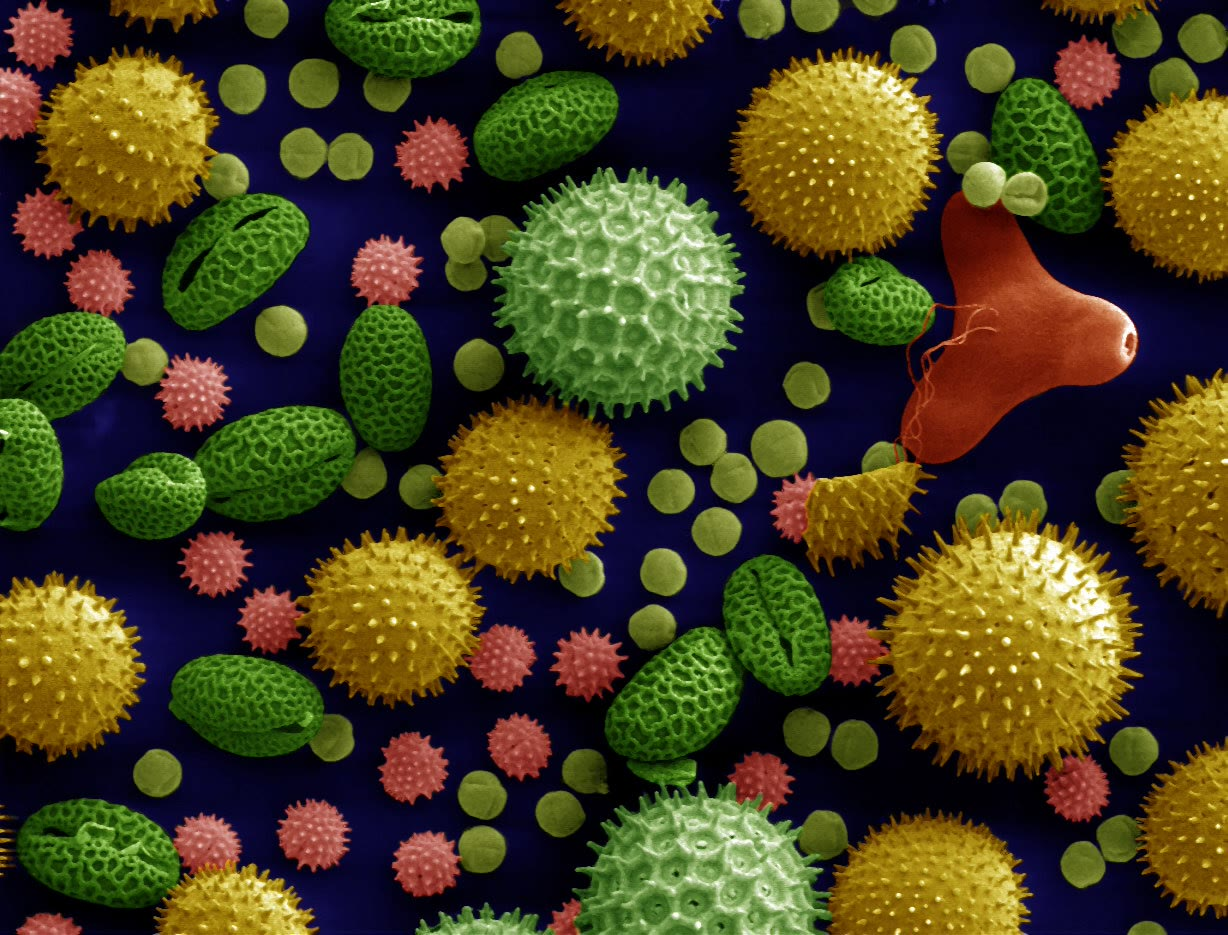
\includegraphics[width=0.46\linewidth]{images/book2/g12-pollen-sem.jpg}

{\small حبوب لقاح خمسة نباتات شائعة (دوار الشمس، والمجد الصباحي،
والخطمي الوردي، والزنبق، وزهرة الربيع) كما تُرى بالمجهر الإلكتروني الماسح،
بألوان زائفة. ولكل نوع من النباتات شكل حبوبه الخاص. مرفق المجهر
الإلكتروني في دارتموث (ملك عام، عبر ويكيميديا كومنز).}
\end{omfigure}
% ledger: photo:g12-pollen

\begin{definition}[تحليل حبوب اللقاح]\label{def:g12:past-climates:pollen}
\emph{تحليل حبوب اللقاح}\index{تحليل حبوب اللقاح} هو قراءة الغطاء النباتي
الماضي من حبوب اللقاح المحفوظة في الرسوبيات: ففي كل طبقة من عينة لبية،
تُعرَّف الحبوب وتُعدّ، وتُرسم حصة كل نوع من النباتات،
بالنسبة المئوية من الحبوب المعدودة، بدلالة العمق في
\emph{مخطط حبوب اللقاح}\index{مخطط حبوب اللقاح}.
\end{definition}
% ledger: ncei:pollen

بدأ عدّ حبوب اللقاح على هذا النحو مع الجيولوجي السويدي لينارت فون
بوست، الذي قدّم أول مخطط حديث لحبوب اللقاح، بالأرقام، في عام 1916؛
ويُظهر مثل هذا المخطط العمق نزولًا على الصفحة ومنحنى لكل نوع من
النباتات. والغطاء النباتي بدوره يحدّث عن المناخ: فالحشائش وغيرها من
الأعشاب مع شبه انعدام الأشجار تعني منظرًا مفتوحًا باردًا، بينما يحتاج البلوط
والبندق إلى صيف دافئ.
% ledger: rull18:von-post; the Varden diagram is invented (ice_age_records.py POLLEN)

\begin{omfigure}
\begin{tikzpicture}
\pgfplotsset{pollen/.style={scale only axis, height=6cm, ymin=300, ymax=600,
  y dir=reverse, xmin=0, axis x line*=bottom, axis y line*=left, axis line style={-},
  tick label style={font=\scriptsize}, title style={font=\small, yshift=-4pt, text depth=0.25ex, text height=1.6ex},
  ytick={300,350,...,600}, xmajorgrids, ymajorgrids,
  grid style={gray!22, line width=0.3pt}}}
\begin{axis}[pollen, name=p1, width=3.0cm, xmax=100, xtick={0,20,...,80}, title={الأعشاب},
  ylabel={\foreignlanguage{arabic}{العمق \babelsublr{(cm)}}}, every axis label/.append style={font=\small}]
\addplot[fill=omLithSand, draw=black!70, line width=0.4pt] table[x=pct, y=depth_cm] {figdata/out/grade-12-ice_age_records-pol-herbs.dat};
\coordinate (z1) at (axis cs:0,550);
\coordinate (z2) at (axis cs:0,470);
\coordinate (z3) at (axis cs:0,425);
\end{axis}
\begin{axis}[pollen, name=p2, at={(p1.south east)}, anchor=south west, xshift=0.3cm,
  width=1.8cm, xmax=60, xtick={0,20,40}, title={البتولا}, yticklabels={}]
\addplot[fill=omHypsLandB, draw=black!70, line width=0.4pt] table[x=pct, y=depth_cm] {figdata/out/grade-12-ice_age_records-pol-birch.dat};
\end{axis}
\begin{axis}[pollen, name=p3, at={(p2.south east)}, anchor=south west, xshift=0.3cm,
  width=1.8cm, xmax=60, xtick={0,20,40}, title={الصنوبر}, yticklabels={}]
\addplot[fill=omHypsLandA, draw=black!70, line width=0.4pt] table[x=pct, y=depth_cm] {figdata/out/grade-12-ice_age_records-pol-pine.dat};
\end{axis}
\begin{axis}[pollen, name=p4, at={(p3.south east)}, anchor=south west, xshift=0.3cm,
  width=1.2cm, xmax=40, xtick={0,20}, title={البندق}, yticklabels={}]
\addplot[fill=omHypsLandD, draw=black!70, line width=0.4pt] table[x=pct, y=depth_cm] {figdata/out/grade-12-ice_age_records-pol-hazel.dat};
\end{axis}
\begin{axis}[pollen, name=p5, at={(p4.south east)}, anchor=south west, xshift=0.3cm,
  width=1.5cm, xmax=50, xtick={0,20,40}, title={البلوط}, yticklabels={}]
\addplot[fill=omHypsLandE, draw=black!70, line width=0.4pt] table[x=pct, y=depth_cm] {figdata/out/grade-12-ice_age_records-pol-oak.dat};
\coordinate (e1) at (axis cs:50,550);
\coordinate (e2) at (axis cs:50,470);
\coordinate (e3) at (axis cs:50,425);
\coordinate (top) at (axis cs:50,300);
\coordinate (bot) at (axis cs:50,600);
\end{axis}
\draw[densely dashed, black!70] (z1) -- (e1 -| p5.east);
\draw[densely dashed, black!70] (z2) -- (e2 -| p5.east);
\draw[densely dashed, black!70] (z3) -- (e3 -| p5.east);
\node[font=\scriptsize, anchor=west] at ($(bot -| p5.east)!0.5!(e1 -| p5.east)$) {\foreignlanguage{arabic}{النطاق 1}};
\node[font=\scriptsize, anchor=west] at ($(e1 -| p5.east)!0.5!(e2 -| p5.east)$) {\foreignlanguage{arabic}{النطاق 2}};
\node[font=\scriptsize, anchor=west] at ($(e2 -| p5.east)!0.5!(e3 -| p5.east)$) {\foreignlanguage{arabic}{النطاق 3}};
\node[font=\scriptsize, anchor=west] at ($(e3 -| p5.east)!0.5!(top -| p5.east)$) {\foreignlanguage{arabic}{النطاق 4}};
\node[font=\scriptsize, anchor=north] at ($(p1.south)!0.5!(p5.south)+(0,-0.45)$) {النسبة المئوية من حبوب اللقاح المعدودة};
\end{tikzpicture}

{\small \omterm{def:g12:past-climates:pollen}{مخطط حبوب اللقاح} لبحيرة في تلال فاردن، المنطقة المتخيَّلة
في هذه السلسلة: بيانات تمرين متخيَّلة، تتبع التعاقب الموجود في كثير من
بحيرات المنطقة المعتدلة الباردة. عمر قاع العينة (\qty{600}{cm})
\num{14000} سنة، وعمر أعلاها المرسوم (\qty{300}{cm}) \num{6000} سنة،
بمعدل ترسيب ثابت بينهما.}
\end{omfigure}
% invented exercise data (ice_age_records.py POLLEN); no ledger row

\begin{method}[قراءة مخطط حبوب اللقاح]
\begin{enumerate}
  \item اقرأ المحور الرأسي: العمق، والطبقات الأقدم في الأسفل؛
        وحوّل الأعماق إلى أعمار بتواريخ العينة.
  \item لكل طبقة، جد النباتات ذات الحصص الأكبر.
  \item قسّم العينة إلى نطاقات، لكل منها مجموعتها الخاصة من النباتات
        السائدة؛ وضع الحدود حيث تتغير المنحنيات أسرع ما يكون.
  \item سمِّ الغطاء النباتي لكل نطاق (أعشاب مفتوحة، أو غابة بتولا، أو غابة
        صنوبر، أو غابة عريضة الأوراق) والمناخ الذي يحتاج إليه.
  \item اقرأ النطاقات من الأسفل إلى الأعلى تاريخًا للمنظر الطبيعي.
\end{enumerate}
\end{method}

في المخطط أعلاه، النطاق 1 منظر من الأعشاب، مع قليل من أشجار البتولا:
البلاد المفتوحة الباردة التي خلّفها الجليد. وفي النطاق 2، ينتشر البتولا أولًا، وهو شجرة
متحمّلة؛ ويتبعه الصنوبر في النطاق 3؛ وفي النطاق 4 يسود البندق والبلوط، اللذان يحتاجان إلى صيف
دافئ. وإذا قُرئت العينة من الأسفل إلى الأعلى، روت نهاية
\omterm{def:g12:past-climates:glacial-cycle}{الفترة الجليدية} وقدوم دفء \omterm{def:g12:past-climates:glacial-cycle}{الفترة بين الجليدية}، إذ
عادت الغابة إلى البلاد.

\section{رسوبيات المحيطات والإيقاع الفلكي}

على قاع المحيط المفتوح، يتراكم الوحل ببطء ودون انقطاع،
طبقة فوق طبقة، ملايين السنين. وهو مليء بأصداف
المنخربات: كائنات وحيدة الخلية صدفتها، التي لا يبلغ عرضها إلا جزءًا من
الملّيمتر، كثيرًا ما تكون من الكالسيت. بعضها يطفو قرب
السطح؛ وبعضها يعيش على قاع البحر.
% ledger: ucmp:forams, lr04:stack (benthic), photo:g12-forams (planktic)

\begin{omfigure}
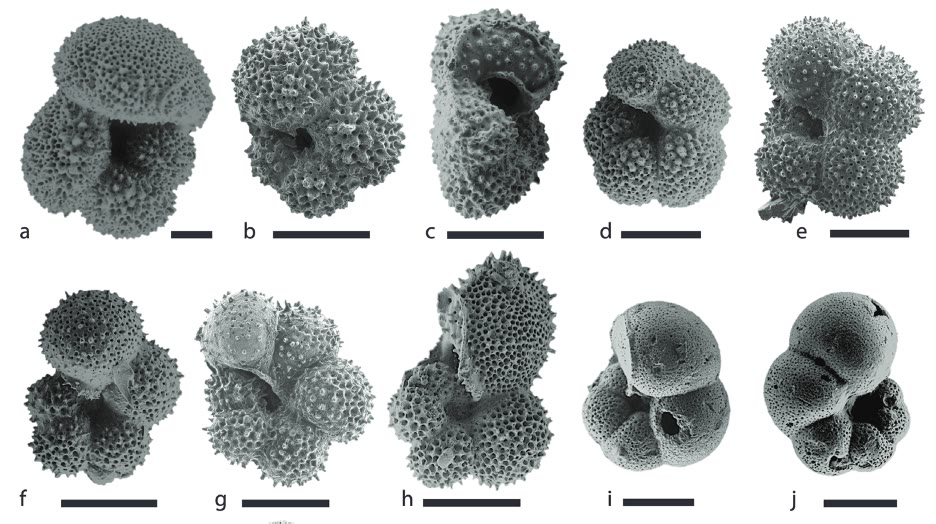
\includegraphics[width=0.62\linewidth]{images/book2/g12-planktic-foraminifera.jpg}

{\small أصداف عشرة أنواع من المنخربات عاشت طافية في
المحيط، كما تُرى بالمجهر الإلكتروني الماسح؛ وطول كل خط مقياس
\qty{150}{\micro\metre}، فكل صدفة في حجم حبة رمل تقريبًا.
مارسي روبنسون، هيئة المسح الجيولوجي الأمريكية (ملك عام، عبر ويكيميديا كومنز).}
\end{omfigure}
% ledger: photo:g12-forams

يأتي أكسجين الصدفة من ماء البحر. فالماء المكوّن من النظير الخفيف
الأكسجين-16 يتبخر أسهل، والثلج الذي يبني الأغطية
الجليدية لذلك فقير بالأكسجين-18. وحين تنمو الأغطية الجليدية، تخزن
هذا الماء الخفيف، فيصير المحيط الباقي أغنى بالأكسجين-18؛ وكذلك
الأصداف التي تنمو فيه، وأكثر كلما كان الماء أبرد. وحصة
الأكسجين-18 في أصداف منخربات قاع البحر، التي تُكتب
$\delta^{18}\mathrm{O}$ وتُعطى بأجزاء من الألف، هي إذن \omterm{def:g12:past-climates:proxy}{مؤشر بديل}
لحجم الجليد على اليابسة ولدرجة حرارة \omterm{def:g10:layered-ocean:thermocline}{المحيط العميق}: فكلما
ارتفعت، زاد الجليد وبرد الماء.
% ledger: nasaeo:o18, lr04:stack

السجل أدناه، المسمّى LR04، يجمع قياسات 57 عينة لبية من جميع
المحيطات في منحنى واحد يغطي 5.3 مليون سنة.

\begin{omfigure}
\begin{tikzpicture}
\begin{axis}[omrecord, scale only axis, width=0.86\linewidth, height=4.8cm,
  xmin=0, xmax=5.32, x dir=reverse, ymin=2.4, ymax=5.3, y dir=reverse,
  xtick={0,0.5,...,5}, ytick={2.5,3,...,5},
  x tick label style={/pgf/number format/.cd, fixed, precision=1},
  y tick label style={/pgf/number format/.cd, fixed, fixed zerofill, precision=1},
  xlabel={\foreignlanguage{arabic}{ملايين السنين قبل عام 1950}},
  ylabel={\foreignlanguage{arabic}{$\delta^{18}\mathrm{O}$ في الأصداف \babelsublr{(\unit{\permil})}}}]
\fill[omProp!14] (axis cs:1.25,2.4) rectangle (axis cs:0.7,5.3);
% data:lr04 (the stack only; ice_age_records.py)
\addplot[omDef!85!black, line width=0.35pt] table[x=age_Ma, y=d18O] {figdata/out/grade-12-ice_age_records-lr04.dat};
\addplot[omThm, line width=1pt, densely dashed, unbounded coords=jump] table[x=age_Ma, y=d18O] {figdata/out/grade-12-ice_age_records-lr04mean.dat};
\coordinate (mpt) at (axis cs:0.975,2.45);
\coordinate (mm) at (axis cs:5.22,4.92);
\coordinate (arr) at (axis cs:5.12,3.9);
\end{axis}
\node[font=\scriptsize, anchor=north, align=center] at (mpt) {\foreignlanguage{arabic}{من \babelsublr{\num{41000}} إلى}\\\foreignlanguage{arabic}{\babelsublr{\num{100000}} سنة}};
\draw[omThm, line width=1pt, densely dashed] (mm) -- ($(mm)+(0.5,0)$) node[right, font=\scriptsize, text=omThm] {\foreignlanguage{arabic}{متوسطا الفترتين من 5.3 إلى 3 ومن 1 إلى 0 مليون سنة مضت}};
\draw[-{Stealth}, black!70] (arr) -- ++(0,-0.9) node[midway, right, font=\scriptsize, align=left] {جليد أكثر\\وبرودة أشد};
\end{tikzpicture}

{\small خمسة ملايين سنة من \omterm{def:g10:layered-ocean:thermocline}{المحيط العميق} في أصداف منخربات
قاع البحر؛ والمحور الرأسي معكوس، كي تكون الأزمنة الباردة الجليدية
في الأسفل. والخطان المتقطعان متوسطا الجزأين الأول والأخير. والمظلل:
التحول من إيقاع دورته \num{41000} سنة إلى إيقاع دورته نحو \num{100000}
سنة. البيانات: ليسيكي ورايمو (2005)، مجموعة LR04.}
\end{omfigure}
% ledger: data:lr04, lr04:stack, clark06:mpt

يقول السجل، إذا قُرئ بالطريقة السابقة، ثلاثة أشياء.
\begin{itemize}
  \item \emph{لقد بردت الأرض ونما جليدها.} فالقيمة المتوسطة
        ترتفع من \qty{3.03}{\permil} بين 5.3 و3 ملايين سنة
        مضت إلى \qty{4.15}{\permil} على مدى المليون سنة الأخيرة.
  \item \emph{لقد كبرت التذبذبات.} فالأزمنة الجليدية والبين جليدية
        تتعاقب على امتداد السجل كله، لكن تذبذبها يتسع أكثر فأكثر: ففي
        \omterm{def:g12:past-climates:lgm}{الذروة الجليدية الأخيرة} كانت القيمة \qty{4.92}{\permil}، مقابل
        \qty{3.23}{\permil} اليوم.
  \item \emph{لقد تغيّر الإيقاع.} فبين 2.6 و1.3 مليون سنة
        مضت، أقوى دورة في السجل، محسوبةً من بياناته، هي
        \num{41000} سنة؛ وعلى مدى \num{700000} السنة الأخيرة هي نحو
        \num{98000} سنة، وهو إيقاع \omterm{def:g12:past-climates:ice-core}{العينات الجليدية}. وقد حدث التحول
        بين نحو 1.25 و0.7 مليون سنة مضت.
\end{itemize}
% ledger: data:lr04, clark06:mpt (ice_age_records.py: lr04_mean_3_5Ma 3.032, lr04_mean_0_1Ma 4.147, lr04_lgm 4.92, lr04_today 3.23, periods 41.0 and 98.5 kyr)

هذه الدورات ليست مصادفة. ففي عام 1976 وجد جيمس هايز وجون إمبري ونيكولاس
شاكلتون في رسوبيات المحيطات الجنوبية ثلاثة إيقاعات، دوراتها
\num{23000} و\num{42000} ونحو \num{100000} سنة، وهي دورات
التغيرات البطيئة في مدار الأرض ومحورها: مبادرة المحور،
وميل المحور (نحو \num{41000} سنة)، وشكل المدار
(نحو \num{100000} سنة). وهذه التغيرات تبدّل ضوء الشمس الذي يتلقاه كل
خط عرض في كل فصل، وتضبط إيقاع \omterm{def:g12:past-climates:glacial-cycle}{الدورات
الجليدية}. أما كيف تفعل ذلك، ولماذا ساد الإيقاع البطيء ذو \num{100000} سنة،
فهو موضوع مقرر جامعي.
% ledger: hays76:periods, nasa:milankovitch, lr04:stack, clark06:mpt

\begin{dated}{2025}
في يناير 2025، أعلن مشروع بيوند إبيكا أن عينة لبية حُفرت في
ليتل دوم~C، على بعد نحو \qty{35}{km} من محطة كونكورديا في دوم~C، تحوي
سجلًا متصلًا يعود إلى نحو 1.2 مليون سنة في أعلى
\qty{2480}{m} منها. وهي تغطي الزمن
الذي تحوّل فيه الإيقاع الجليدي من \num{41000} إلى \num{100000} سنة،
ويجري تحليل الجليد وهوائه.
\end{dated}
% ledger: ku25:beyond-epica, ipev25:little-dome-c

\section{مناخات الزمن السحيق}

قبل زمن \omterm{def:g12:past-climates:ice-core}{العينات الجليدية}، تُقرأ مناخات الماضي من
الرسوبيات، والأوراق والتربات الأحفورية، والنظائر. وقد اختارت الهيئة الحكومية الدولية المعنية بتغير المناخ بضع
\emph{فترات مرجعية}، مدروسة جيدًا، تساعد مناخاتها على تقدير
تغيرات اليوم والغد. ويعطي المخطط أدناه درجة حرارتها العالمية
عند السطح، مقارنةً بالفترة 1850--1900.

\begin{omfigure}
\begin{tikzpicture}
\begin{axis}[omrecord, width=0.86\linewidth, height=5.4cm, xmin=-9, xmax=27,
  ymin=0.4, ymax=6.6, y dir=reverse, ytick={1,...,6}, ymajorgrids=false,
  yticklabels={{\foreignlanguage{arabic}{\mbox{\textdir TLT PETM}، \mbox{\textdir TLT 56} مليون سنة}}, {\foreignlanguage{arabic}{\mbox{\textdir TLT EECO}، \mbox{\textdir TLT 53}--\mbox{\textdir TLT 49} مليون سنة}}, {\foreignlanguage{arabic}{\mbox{\textdir TLT MPWP}، \mbox{\textdir TLT 3.3}--\mbox{\textdir TLT 3.0} مليون سنة}},
    {\foreignlanguage{arabic}{\mbox{\textdir TLT LIG}، \mbox{\textdir TLT 129}--\mbox{\textdir TLT 116} ألف سنة}}, {\foreignlanguage{arabic}{\mbox{\textdir TLT LGM}، \mbox{\textdir TLT 23}--\mbox{\textdir TLT 19} ألف سنة}}, {\foreignlanguage{arabic}{\mbox{\textdir TLT MH}، \mbox{\textdir TLT 6.5}--\mbox{\textdir TLT 5.5} ألف سنة}}},
  y tick label style={font=\scriptsize},
  xlabel={\foreignlanguage{arabic}{درجة الحرارة مقارنةً بالفترة 1850--1900 \babelsublr{(\unit{\degreeCelsius})}}}]
% ipcc:fig2-34 (DEEP in ice_age_records.py)
\addplot[draw=none, mark=none, restrict expr to domain={\thisrow{tlo}}{0:30},
  error bars/.cd, x dir=both, x explicit,
  error bar style={line width=5pt, omWarm!75}, error mark=none]
  table[x expr={(\thisrow{tlo}+\thisrow{thi})/2}, y=idx,
        x error expr={(\thisrow{thi}-\thisrow{tlo})/2}] {figdata/out/grade-12-ice_age_records-deep.dat};
\addplot[draw=none, mark=none, restrict expr to domain={\thisrow{tlo}}{-30:-0.01},
  error bars/.cd, x dir=both, x explicit,
  error bar style={line width=5pt, omCold!75}, error mark=none]
  table[x expr={(\thisrow{tlo}+\thisrow{thi})/2}, y=idx,
        x error expr={(\thisrow{thi}-\thisrow{tlo})/2}] {figdata/out/grade-12-ice_age_records-deep.dat};
\draw[black!60] (axis cs:0,0.4) -- (axis cs:0,6.6);
\draw[omThm, densely dashed, line width=0.8pt] (axis cs:1.09,0.4) -- (axis cs:1.09,6.6);
\node[font=\scriptsize, text=omThm, anchor=west, fill=white, inner sep=1pt] at (axis cs:1.6,4.55) {2011--2020};
\end{axis}
\end{tikzpicture}

{\small درجة الحرارة العالمية عند السطح لست فترات مرجعية من الماضي،
ومداها المرجح جدًا، مقارنةً بالفترة 1850--1900؛ والخط المتقطع: العقد 2011--2020.
PETM: الحد الأقصى الحراري للباليوسين--الإيوسين؛ EECO: الأمثل المناخي للإيوسين
المبكر؛ MPWP: الفترة الدافئة في منتصف البليوسين؛ LIG: آخر \omterm{def:g12:past-climates:glacial-cycle}{فترة بين جليدية}؛ LGM: \omterm{def:g12:past-climates:lgm}{الذروة
الجليدية الأخيرة}، وهي الفترة الباردة الوحيدة (بالأزرق)؛ MH:
منتصف الهولوسين. القيم: تقرير التقييم السادس، الفريق العامل الأول، الشكل 2.34.}
\end{omfigure}
% ledger: ipcc:fig2-34, ipcc:gsat-2011-2020, ipcc:ref-periods

\begin{center}
\small
\begin{tabular}{|l|c|c|c|}
\hline
\textbf{الفترة} & \textbf{درجة الحرارة (\unit{\degreeCelsius})} & \textbf{ثاني أكسيد الكربون (ppm)} & \textbf{مستوى البحر (m)} \\
\hline
\mbox{\textdir TLT PETM}، 56 مليون سنة & من $+10$ إلى $+25$ & نحو 900، يرتفع إلى 2000 & --- \\
\mbox{\textdir TLT EECO}، 53--49 مليون سنة & من $+10$ إلى $+18$ & من 1150 إلى 2500 & من $+70$ إلى $+76$ \\
\mbox{\textdir TLT MPWP}، 3.3--3.0 مليون سنة & من $+2.5$ إلى $+4.0$ & من 360 إلى 420 & من $+5$ إلى $+25$ \\
\mbox{\textdir TLT LIG}، 129--116 ألف سنة & من $+0.5$ إلى $+1.5$ & من 266 إلى 282 & من $+5$ إلى $+10$ \\
\textcolor{omCold}{\mbox{\textdir TLT LGM}، 23--19 ألف سنة} & \textcolor{omCold}{من $-7$ إلى $-5$} & \textcolor{omCold}{من 188 إلى 194} & \textcolor{omCold}{من $-134$ إلى $-125$} \\
\mbox{\textdir TLT MH}، 6.5--5.5 ألف سنة & من $+0.2$ إلى $+1.0$ & من 260 إلى 268 & من $-3.5$ إلى $+0.5$ \\
\hline
\end{tabular}

\medskip
{\small الفترات المرجعية: درجة الحرارة العالمية عند السطح مقارنةً بالفترة
1850--1900، وثاني أكسيد الكربون، والمتوسط العالمي لمستوى البحر مقارنةً بعام 1900. تقرير
التقييم السادس، الفريق العامل الأول، الشكل 2.34.}
\end{center}
% ledger: ipcc:fig2-34

كان الحد الأقصى الحراري للباليوسين--الإيوسين احترارًا مفاجئًا، حين بلغت دفعة كبيرة
من الكربون المحيط والهواء: فصار المحيط أكثر حمضية
وأفقر بالأكسجين، وانقرضت أنواع كثيرة من أعماق البحار. وفي الأمثل المناخي
للإيوسين المبكر، بقي ثاني أكسيد الكربون فوق \qty{1000}{ppm} ملايين
السنين، ولم يكن هناك جليد قطبي، ونمت غابات قريبة من الغابات المدارية
عند خط العرض \ang{70} جنوبًا. والفترة الدافئة في منتصف البليوسين هي آخر مرة كان فيها ثاني أكسيد
الكربون قريبًا من مستواه اليوم: فقد كان القطب الشمالي أدفأ بكثير مما هو الآن، وكان البحر
أعلى. وفي آخر \omterm{def:g12:past-climates:glacial-cycle}{فترة بين جليدية}، كان الغطاءان الجليديان لغرينلاند ولغرب القارة القطبية الجنوبية
أصغر والبحر أعلى مما اليوم، وعاشت أفراس النهر
في بريطانيا.
% ledger: ipcc:ref-periods, ipcc:fig2-34, ipcc:mpwp-eeco

تضع هذه الأرشيفات الحاضر في منظوره، والهيئة الحكومية الدولية تعقد المقارنة
بنفسها. ففي عام 2019 كان ثاني أكسيد الكربون في الهواء أعلى مما كان في أي وقت خلال
مليوني سنة على الأقل (\emph{بثقة عالية})، والزيادات في ثاني أكسيد
الكربون والميثان منذ عام 1750 تتجاوز بكثير التغيرات الطبيعية بين \omterm{def:g12:past-climates:glacial-cycle}{الفترات الجليدية}
والبين جليدية على مدى \num{800000} سنة على الأقل (\emph{بثقة عالية
جدًا}). وقد ارتفعت درجة الحرارة العالمية عند السطح منذ عام 1970 أسرع مما ارتفعت
في أي فترة أخرى من 50 سنة خلال \num{2000} السنة الأخيرة على الأقل
(\emph{بثقة عالية}). وكان العقد 2011--2020 أدفأ من أدفأ
قرون \omterm{def:g12:past-climates:glacial-cycle}{الفترة بين الجليدية} الحالية، قبل نحو \num{6500} سنة، وقريبًا
من دفء آخر \omterm{def:g12:past-climates:glacial-cycle}{فترة بين جليدية}، قبل نحو \num{125000} سنة
(\emph{بثقة متوسطة}).
% ledger: ipcc:co2-ch4-800kyr, ipcc:fastest-2000yr, ipcc:co2-2myr

ويمكن مقارنة سرعة التغير أيضًا. فمن 1970 إلى 2025، يبلغ اتجاه
سجل درجة الحرارة العالمية \qty{0.20}{\degreeCelsius} لكل عقد، أي
نحو \qty{20}{\degreeCelsius} لكل ألف سنة لو استمر؛ أما
الاحترار الخارج من \omterm{def:g12:past-climates:glacial-cycle}{الفترة الجليدية} الأخيرة فكان متوسطه نحو
\qty{0.86}{\degreeCelsius} لكل ألف سنة. وأسباب تغير اليوم،
وما قد يصير إليه، موضوع \cref{ch:g12:climate-change}.
% ledger: data:gistemp (ice_age_records.py: rate_1970_2025_C_per_decade 0.2012), ipcc:lgm-cooling, ipcc:ref-periods

\section{تمارين}

\begin{exercise}[$\star$]\label{exo:g12:past-climates:1}
أعطِ المصطلح: (أ) كمية تُقاس في أرشيف وتقوم مقام
متغير مناخي لم يُقس؛ (ب) أسطوانة من الجليد تُستخرج بالحفر من غطاء جليدي؛
(ج) فترة دافئة بين \omterm{def:g12:past-climates:glacial-cycle}{فترتين جليديتين}؛ (د) قراءة الغطاء النباتي الماضي
من حبوب اللقاح الأحفورية؛ (ه) الزمن، قبل نحو \num{23000} إلى \num{19000}
سنة، الذي كانت فيه آخر الأغطية الجليدية في أكبر امتداد لها.
\end{exercise}

\begin{exercise}[$\star$]\label{exo:g12:past-climates:2}
لكل \omterm{def:g12:past-climates:proxy}{مؤشر بديل}، سمِّ أرشيفه وما يخبر عنه: (أ) الهواء في
الفقاعات؛ (ب) حصة حبوب لقاح البلوط؛ (ج) الأكسجين-18 في أصداف
منخربات قاع البحر؛ (د) عرض حلقات الأشجار.
\end{exercise}

\begin{exercise}[$\star$]\label{exo:g12:past-climates:3}
في أثناء مرحلة انحسار الجليد الأخيرة، من نحو \num{18000} إلى \num{11000}
سنة مضت، ارتفع مستوى سطح البحر من نحو \qty{-120}{m} إلى \qty{-50}{m}. (أ) احسب
متوسط معدل الارتفاع، بالملّيمترات في السنة. (ب) من 2006 إلى 2018، ارتفع مستوى
سطح البحر بمقدار \qty{3.7}{mm} في السنة. قارن.
\end{exercise}

\begin{exercise}[$\star$]\label{exo:g12:past-climates:4}
ارتفعت درجة الحرارة العالمية بمقدار \qty{0.20}{\degreeCelsius} لكل عقد من
1970 إلى 2025. عبّر عن هذا المعدل لكل قرن ولكل ألف سنة.
\end{exercise}

\begin{exercise}[$\star$]\label{exo:g12:past-climates:5}
وجد هايز وإمبري وشاكلتون ثلاثة إيقاعات في رسوبيات المحيطات:
\num{23000} و\num{42000} ونحو \num{100000} سنة. (أ) طابق كلًّا منها مع
مبادرة المحور، وميل المحور، وشكل المدار.
(ب) كم دورة من \num{41000} سنة تتسع لها \num{1000000} سنة؟ وكم
دورة من \num{100000} سنة؟
\end{exercise}

\begin{exercise}[$\star\star$]\label{exo:g12:past-climates:6}
خط المربعات الصغرى في الفصل هو $\mathrm{CO_2} \approx 266.6 +
7.83\,\Delta T$ (بوحدة ppm، و$\Delta T$ بوحدة \unit{\degreeCelsius}).
(أ) تنبأ بثاني أكسيد الكربون لمتوسط درجة حرارة \omterm{def:g12:past-climates:lgm}{الذروة الجليدية
الأخيرة} في دوم~C، \qty{-9.4}{\degreeCelsius}، وقارن بالقيمة المقيسة
\qty{190}{ppm}. (ب) تنبأ به لأدفأ نقطة، \qty{+5.5}{\degreeCelsius}،
وقارن بأعلى قيمة مقيسة، \qty{299}{ppm}. (ج) استعمل الخط
لتقدير درجة حرارة دوم~C التي توافق \qty{427}{ppm}، وهي
قيمة عام 2025 في ماونا لوا. لماذا لا يكون هذا الاستعمال الأخير للخط مسوَّغًا؟
\end{exercise}

\begin{exercise}[$\star\star$]\label{exo:g12:past-climates:7}
استعمل \omterm{def:g12:past-climates:pollen}{مخطط حبوب اللقاح} لبحيرة تلال فاردن. (أ) ما حبوب اللقاح
السائدة عند \qty{580}{cm}، وأي منظر طبيعي تدل عليه؟ (ب) السؤال نفسه
عند \qty{340}{cm}. (ج) أي شجرة تنتشر أولًا بعد البرد،
وأي الأشجار تصل أخيرًا؟ (د) لماذا قد يتأخر وصول شجرة عن
الاحترار الذي سمح به؟
\end{exercise}

\begin{exercise}[$\star\star$]\label{exo:g12:past-climates:8}
في العينة نفسها، عمر الوحل عند \qty{600}{cm} \num{14000} سنة، وعمره
عند \qty{300}{cm} \num{6000} سنة، بمعدل ترسيب ثابت.
(أ) احسب هذا المعدل بالملّيمترات في السنة. (ب) جد عمر الحد
بين النطاقين 2 و3، عند \qty{470}{cm}. (ج) كم سنة تمثل شريحة
سمكها \qty{1}{cm}؟
\end{exercise}

\begin{exercise}[$\star\star$]\label{exo:g12:past-climates:9}
على خريطة جنوب شرق آسيا، تزداد اليابسة فوق البحر من 4.11 إلى
7.16 مليون كيلومتر مربع حين يُخفض البحر بمقدار \qty{130}{m}.
(أ) احسب الزيادة ونسبتها المئوية. (ب) على الخريطة، يكفي انخفاض بنحو
\qty{36}{m} لوصل بورنيو بآسيا. هل كانت الجزيرة متصلة طوال \omterm{def:g12:past-climates:lgm}{الذروة الجليدية
الأخيرة}؟ فسّر. (ج) لماذا خط ساحل الخريطة تقريبي
فقط؟
\end{exercise}

\begin{exercise}[$\star\star$]\label{exo:g12:past-climates:10}
في سجل LR04، القيمة في \omterm{def:g12:past-climates:lgm}{الذروة الجليدية الأخيرة}
\qty{4.92}{\permil} وقيمة اليوم \qty{3.23}{\permil}. (أ) أيهما الأعلى،
وهل هذا ما تتوقعه؟ فسّر بالأغطية الجليدية. (ب) لماذا يُرسم
المحور الرأسي للسجل معكوسًا؟
\end{exercise}

\begin{exercise}[$\star\star$]\label{exo:g12:past-climates:11}
يقول صديق: «الارتباط البالغ 0.92 بين درجة حرارة القارة القطبية الجنوبية
وثاني أكسيد الكربون يثبت أن ثاني أكسيد الكربون هو الذي تحكّم في العصور الجليدية».
(أ) ماذا يُظهر الارتباط، وماذا لا يُظهر؟ (ب) أعطِ تفسيرين
آخرين يعطيان الارتباط نفسه. (ج) أي نوع من
المعلومات عن السجلين يساعد على الحسم؟
\end{exercise}

\begin{exercise}[$\star\star\star$]\label{exo:g12:past-climates:12}
أقوى دورة في سجل LR04 هي \num{41000} سنة بين 2.6
و1.3 مليون سنة مضت، و\num{98500} سنة على مدى \num{700000} السنة
الأخيرة. (أ) كم دورة تحوي كل نافذة؟ (ب) أي تغير في
مدار الأرض أو محورها يوافق كل دورة؟ (ج) فسّر لماذا يستطيع سجل فيه
عينة واحدة كل \num{2000} سنة أن يُظهر هذه الإيقاعات، لكن لا يستطيع أن يُظهر تغيرًا
دام قرنًا.
\end{exercise}

\begin{exercise}[$\star\star\star$]\label{exo:g12:past-climates:13}
كان معدل ارتفاع ثاني أكسيد الكربون من 192 إلى \qty{198}{ppm} لكل قرن في
1995--2014. وفي أثناء الحد الأقصى الحراري للباليوسين--الإيوسين كان من 4 إلى
\qty{42}{ppm} لكل قرن، وفي أثناء مرحلة انحسار الجليد الأخيرة لم يتجاوز
نحو \qty{10}{ppm} لكل قرن. (أ) كم مرة كان الارتفاع الحديث أسرع
من أسرع ارتفاع في آخر انحسار للجليد؟ (ب) ومن أبطأ تقديرات
الحد الأقصى الحراري وأسرعها؟ (ج) ارتفع ثاني أكسيد الكربون في الحد الأقصى الحراري من نحو 900 إلى نحو
\qty{2000}{ppm}. كم كان ذلك سيستغرق بمعدل \qty{42}{ppm} لكل قرن،
وبمعدل اليوم؟
\end{exercise}

\begin{exercise}[$\star\star\star$]\label{exo:g12:past-climates:14}
تقدّر الهيئة الحكومية الدولية أن درجة الحرارة العالمية ارتفعت بمقدار 1 إلى
\qty{1.5}{\degreeCelsius} لكل ألف سنة في أسرع أجزاء آخر
انحسار للجليد، وأنها ارتفعت فوق غرينلاند أسرع بنحو عشر مرات في
قرون الاحترار الأسرع. (أ) أعطِ معدل غرينلاند بوحدة
\unit{\degreeCelsius} لكل ألف سنة ولكل عقد. (ب) قارنه
بالمعدل العالمي اليوم البالغ \qty{0.20}{\degreeCelsius} لكل عقد. (ج) لماذا يجب ألا
يُقارن معدل محلي بمعدل عالمي مقارنةً مباشرة؟
\end{exercise}

\begin{exercise}[$\star\star\star$]\label{exo:g12:past-climates:15}
كان مستوى سطح البحر نحو \qty{-50}{m} قبل \num{11000} سنة؛ افترض أنه
ارتفع بعد ذلك بمعدل ثابت قدره \qty{12}{m} لكل ألف سنة، وهو متوسط معدل
الانحسار الرئيسي للجليد. (أ) متى تجاوز \qty{-36}{m}، المستوى الذي يصل بورنيو
بآسيا على الخريطة؟ (ب) بعد ذلك الوقت، هل كان يمكن لشخص أن يمشي من بورنيو إلى
شبه جزيرة الملايو؟ (ج) كم كان البحر سيستغرق ليرتفع
\qty{36}{m} الأخيرة، لو استمر بالسرعة نفسها؟
\end{exercise}

\begin{problem}[{مسألة نهاية الأسبوع --- \num{800000} سنة من جليد القارة القطبية الجنوبية}]
\label{pb:g12:past-climates:1}
% ledger: data:edc-jouzel, data:co2-bereiter, data:lr04, data:gistemp, ipcc:lgm-cooling, ipcc:ref-periods, hays76:periods, clark06:mpt
% values (ice_age_records.py): edc -10.58 / +5.46, co2 173.71 / 298.6, r 0.9165, fit 266.57 + 7.827 T,
% LGM -9.389 / 189.67, 11-9 ka -0.360 / 264.10, period 97.5, rate 0.2012 per decade, ratio 23.48
يعطي جليد دوم~C والهواء الذي في فقاعاته القيم التالية.
ودرجة الحرارة هي التغير فوق الجليد مقارنةً بالألف سنة الأخيرة.

\begin{center}
\small
\begin{tabular}{|l|c|c|}
\hline
 & \textbf{تغير درجة الحرارة (\unit{\degreeCelsius})} & \textbf{ثاني أكسيد الكربون (ppm)} \\
\hline
أبرد قيمة، قبل نحو \num{24000} سنة & $-10.6$ & --- \\
أدفأ قيمة، قبل نحو \num{129000} سنة & $+5.5$ & --- \\
أدنى قيمة لثاني أكسيد الكربون وأعلاها & --- & 174 و299 \\
المتوسط، من \num{23000} إلى \num{19000} سنة مضت & $-9.4$ & 190 \\
المتوسط، من \num{11000} إلى \num{9000} سنة مضت & $-0.4$ & 264 \\
\hline
\end{tabular}
\end{center}

أقوى دورة في سجل درجة الحرارة نحو \num{98000} سنة،
والأزواج البالغة 1639 من القيم تعطي معامل ارتباط قدره 0.92.

\medskip
\noindent\textbf{الجزء الأول --- قراءة السجلين.}
\begin{enumerate}
  \item أي جزء من الجليد يسجل درجة الحرارة، وأيها يسجل
        ثاني أكسيد الكربون؟
  \item احسب المدى الكامل لتغير درجة الحرارة في دوم~C.
  \item احسب المدى الكامل لثاني أكسيد الكربون.
  \item ماذا يقول معامل ارتباط قدره 0.92 عن
        السجلين؟
  \item في الشكل ذي المحور الزمني في الفصل، الحاضر في اليمين. لماذا
        يجب أن تتحقق من الاتجاه الذي يجري فيه الزمن قبل قراءة مثل هذا الشكل؟
\end{enumerate}

\medskip
\noindent\textbf{الجزء الثاني --- القيم الجليدية والبين جليدية.}
\begin{enumerate}[resume]
  \item عرّف \omterm{def:g12:past-climates:glacial-cycle}{الفترة الجليدية} \omterm{def:g12:past-climates:glacial-cycle}{والفترة بين الجليدية}.
  \item في أي الاثنتين نعيش، ومنذ متى؟
  \item كم دورة من \num{98000} سنة تتسع لها \num{800000} سنة؟
  \item أي تغير في مدار الأرض دورته قريبة من
        \num{100000} سنة؟
  \item قبل نحو 1.25 مليون سنة، ما كان الإيقاع الرئيسي
        \omterm{def:g12:past-climates:glacial-cycle}{للدورات الجليدية}؟
\end{enumerate}

\medskip
\noindent\textbf{الجزء الثالث --- آخر انحسار للجليد.}
\begin{enumerate}[resume]
  \item بكم ارتفعت درجة الحرارة فوق دوم~C بين \omterm{def:g12:past-climates:lgm}{الذروة
        الجليدية الأخيرة} والفترة من \num{11000} إلى \num{9000} سنة مضت؟
  \item بكم ارتفع ثاني أكسيد الكربون في الفترة نفسها؟
  \item كانت درجة الحرارة العالمية في \omterm{def:g12:past-climates:lgm}{الذروة الجليدية الأخيرة} أدنى بمقدار 5 إلى
        \qty{7}{\degreeCelsius} من درجة حرارة 1850--1900. خذ منتصف
        هذا المدى. هل تغير القارة القطبية الجنوبية أكبر أم أصغر؟
  \item دامت مرحلة انحسار الجليد الأخيرة من \num{18000} إلى
        \num{11000} سنة مضت. كم تبلغ مدتها؟
  \item احسب متوسط معدل الاحترار العالمي في أثناء المرحلة، بوحدة
        \unit{\degreeCelsius} لكل ألف سنة.
  \item عبّر عن هذا المعدل بوحدة \unit{\degreeCelsius} لكل عقد.
\end{enumerate}

\medskip
\noindent\textbf{الجزء الرابع --- مقارنة معدل اليوم.}
\begin{enumerate}[resume]
  \item من 1970 إلى 2025 ارتفعت درجة الحرارة العالمية بمقدار
        \qty{0.20}{\degreeCelsius} لكل عقد. عبّر عن هذا المعدل لكل
        ألف سنة.
  \item كم مرة يكون احترار اليوم أسرع من متوسط احترار
        آخر انحسار للجليد؟
  \item في أسرع أجزاء انحسار الجليد، ارتفعت درجة الحرارة العالمية
        بمقدار 1 إلى \qty{1.5}{\degreeCelsius} لكل ألف سنة. كم مرة
        يكون معدل اليوم أسرع من هذين؟
  \item استنتج: كم مرة يكون الاحترار العالمي اليوم أسرع من الاحترار الخارج من آخر
        عصر جليدي؟
\end{enumerate}
\end{problem}
